% --------------------------------------------------------------- %
%                       1. TIEKIMO GRANDINĖ                           
% --------------------------------------------------------------- %

\section {Tiekimo grandinė}

Tam, kad galėtume nagrinėti technologijų taikymą tiekimo grandinėse, mums reikia suprasti dalykinę sritį, t.y. kokios yra svarbiausios sąvokos, kokia svarba, mastas, vyraujančios problemos, keliami reikalavimai. Dėl to iš pradžių apžvelgsime šiuos aspektus tolimesniuose poskyriuose.



% --------------------------------------------------------------- %
%                           1.1. SĄVOKA                           
% --------------------------------------------------------------- %

\subsection{Sąvoka}

Tiksliai ir vienareikšmiškai apibrėžti tiekimo grandinę (angl. \textit{Supply chain}) yra ganėtinai sunkus uždavinys. Apskritai, tai yra pakankamai abstrakti sąvoka, kuri gali keistis nuo konteksto, kuriame yra naudojama ir kuri laikui bėgant nemažai evoliucionavo. Pavyzdžiui, grupė akademikų tiekimo grandinę apibrėžė kaip tris arba daugiau šalis, tiesiogiai susijusias su produktų, paslaugų, finansų ir informacijos judėjimo srautais nuo šaltinio iki kliento \cite{mentzer2001defining}. Tuo tarpu Martin Cristopher tiekimo grandinę įvardijo kaip dalyvaujančių organizacijų tinklą, kuris skirtingais procesais ir veiklomis kuria vertę produktų ir paslaugų pavidalu vartotojui \cite{christopher2016logistics}. 

Taip pat Martin Cristopher savo knygoje diskutuoja, kad tiekimo grandinės sąvokoje žodis „tiekimo“ turėtų būti pakeistas žodžiu „paklausos“ (angl. \textit{Demand}), o žodis „grandinė“ žodžiu „tinklas“ (angl. \textit{Network}). Paklausos sąvoka argumentuojama tuo, kad tiekimo grandinė priklauso ne nuo tiekėjų, o nuo rinkos situacijos, t.y paklausos, na o žodis „tinklas“ labiau atspindėtų realybę, kadangi paprastai yra daugiau nei vienas tiekėjas ir klientas. Tokiu būdu tiekimo grandinės modelis (žr. 1 pav.) taptų panašesnis į paklausos tinklo modelį (žr. 2 pav.).

Nors tinklo modelis yra arčiau realybės, dėl paprastumo ir platesnio sąvokos žinomumo šiame darbe vis dėlto naudosime tiekimo grandinės sąvoką turėdami galvoje tinklo struktūrą. Taigi, pasinaudoję abiem moksliniais šaltiniais, galime suformuluoti išvestinį tiekimo grandinės apibrėžimą - tai organizacijų, procesų, paslaugų, finansų ir informacijos visuma, dalyvaujanti produkto gyvavimo cikle nuo pradinio tiekėjo iki galutinio kliento.

\begin{figure}[H]
    \centering
    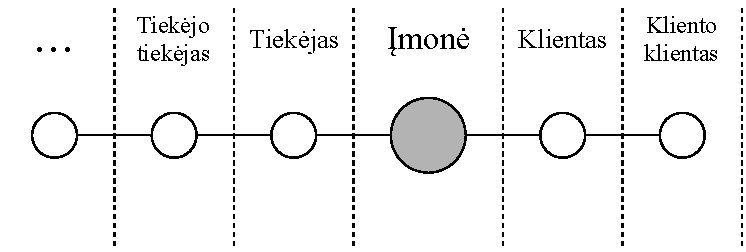
\includegraphics[scale=1]{images/client-supplier-model}
    \caption{Klientų ir tiekėjų sąryšis tiekimo grandinėje}
\end{figure}

Daugelyje mokslinių straipsnių galime aptikti sąvokas „prieš srovę“ (angl. \textit{Upstream}) ir „pasroviui“ (angl. \textit{Downstream}) \cite{croson2005upstream} \cite{frohlich2001arcs} \cite{vachon2006extending}. Tiekimo grandinės kontekste šie žodžiai reiškia įmonės sąryšį su tiekėjais ir klientais. Pavyzdžiui, viską, kas ateina į įmonę iš tiekėjų, paprastai ateina prieš srovę. Tuo tarpu tai, kas išeina iš įmonės pas klientus, atvirkščiai, pasroviui \cite{christopher2016logistics} (žr. 3 pav.). Vėliau įsitikinsime, kad prieš srovę ir pasroviui gali judėti ne tik prekės, bet ir pinigai, informacija ir t.t.

\begin{figure}[H]
    \centering
    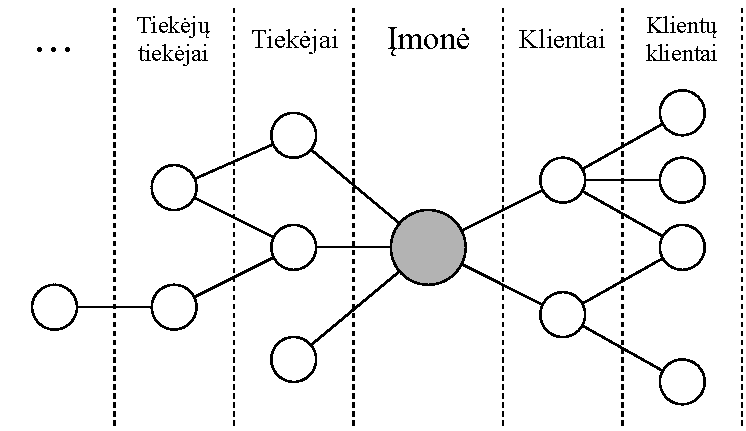
\includegraphics[scale=1]{images/demand-network-model}
    \caption{Paklausos tinklo modelis}
\end{figure}

\begin{figure}[H]
    \centering
    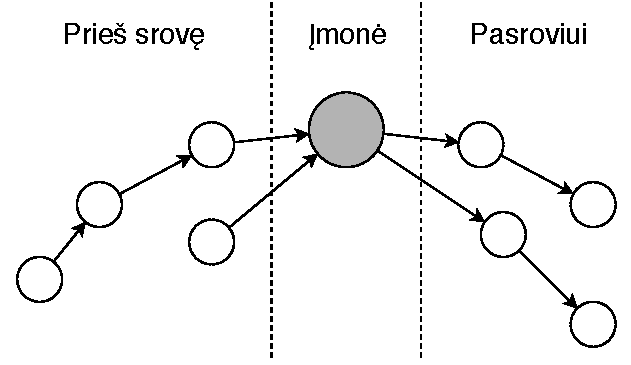
\includegraphics[scale=1]{images/supply-chain-upstream-downstream}
    \caption{Įmonės sąryšiai su tiekėjais ir klientais}
\end{figure}



% --------------------------------------------------------------- %
%                          1.2. STRUKTŪRA                           
% --------------------------------------------------------------- %

\subsection{Struktūra}

Nagrinėdami tiekimo grandinės sąvoką sužinojome, kad yra tiekėjų, klientų ir įmonės rolės. Tačiau tai pernelyg abstraktus modelis, kuris nesuteikia gilesnių žinių apie tiekimo grandinės veikimą. Mums svarbu suprasti kas yra tie tiekėjai, ir klientai, kaip šalys bendrauja tarpusavyje, kokios veiklos ir procesai vyksta tiekimo grandinėje. 

Tačiau visa tai labai priklauso ir nuo industrijų, kuriose šios tiekimo grandinės funkcionuoja. Juk procesai ir praktikos, naudojamos maisto pramonėje nebūtinai gali tikti automobilių gamybos industrijoje. Tą patvirtina vien saugumo klausimų skirtumai tarp šių pramonių \cite{marucheck2011product}.

Nagrinėti tikslią realybėje egzistuojančią tiekimo grandinės struktūrą yra sunku ir dėl to, kad įmonės neviešina savo tiekimo grandinės tikslaus gyvavimo ciklo dėl konfidencialumo ir konkurencijos priežasčių. Tačiau moksliniuose ir internetiniuose šaltiniuose\footnote{https://www2.deloitte.com/content/dam/Deloitte/lu/Documents/technology/lu-blockchain-internet-things-supply-chain-traceability.pdf. Tikrinta 2019-02-11} \footnote{https://www.agric.wa.gov.au/newsletters/ovineobserver/ovine-observer-october-2016-76?page=0\%2C2. Tikrinta 2019-02-11} \footnote{https://www.cflex.com/responsibility/social-responsibility/life-cycle-assessment. Tikrinta 2019-02-11} \footnote{https://www.digitalhealth.gov.au/get-started-with-digital-health/what-is-digital-health/supply-chain/life-cycle-of-a-product. Tikrinta 2019-02-11} galime aptikti nemažai pavyzdinių realybę atspindinčių modelių nuo pat žaliavų surinkimo iki pagaminto produkto pristatymo galutiniam pirkėjui \cite{christopher2016logistics} \cite{webber2009building}. Pasinaudoję jais pabandysime sumodeliuoti savo tiekimo grandinę.

[Pabandykime aprašyti įsivaizduojamos įmonės, gaminančios X pavyzdinį tiekimo grandinės scenarijų. Svarbi vieta - pavyzdį naudosiu visame darbe kituose skyriuose jį atnaujinant ir pagerinant su IoT ir DLT. Svarbu sudaryti tokį modelį tokioje industrijoje, kuris leistų atskleisti gerąsias DLT praktikas ir savybes.] 

[Nupasakoti kas vyksta modelyje, svarbiausias vietas paaiškinti]

[Struktūroje pristatyti pinigų, informacijos, reikalavimų ir prekių srautus]



% --------------------------------------------------------------- %
%                    1.3. SVARBA IR INDUSTRIJOS                           
% --------------------------------------------------------------- %

\subsection{Svarba ir industrijos}



% --------------------------------------------------------------- %
%                   1.4. ŠIANDIENINĖS PROBLEMOS                           
% --------------------------------------------------------------- %

\subsection{Šiandieninės problemos}